\documentclass[a4paper,11pt,twoside]{memoir}

\setcounter{secnumdepth}{2} % Niveau de profondeur pour la numérotation

\let\STARTCODE\relax 
\let\STOPCODE\relax 
\STARTCODE
\usepackage{color,calc,graphicx,soul}
\definecolor{nicered}{rgb}{.647,.129,.149} \makeatletter
\newlength\dlf@normtxtw \setlength\dlf@normtxtw{\textwidth}
\def\myhelvetfont{\def\sfdefault{mdput}} \newsavebox{\feline@chapter}
\newcommand\feline@chapter@marker[1][4cm]{%
  \sbox\feline@chapter{%
    \resizebox{!}{#1}{\fboxsep=1pt%
      \colorbox{nicered}{\color{white}\bfseries\sffamily\thechapter}%
    }}%
  \rotatebox{90}{%
    \resizebox{%
      \heightof{\usebox{\feline@chapter}}+\depthof{\usebox{\feline@chapter}}}%
    {!}{\scshape\so\@chapapp}}\quad%
  \raisebox{\depthof{\usebox{\feline@chapter}}}{\usebox{\feline@chapter}}%
} \newcommand\feline@chm[1][4cm]{%
  \sbox\feline@chapter{\feline@chapter@marker[#1]}%
  \makebox[0pt][l]{% aka \rlap
    \makebox[1cm][r]{\usebox\feline@chapter}%
  }} \makechapterstyle{daleif1}{
%   \setlength{\beforechapskip}{0pt}
%   \setlength{\midchapskip}{0pt}
  \setlength{\afterchapskip}{10pt}
%   \setlength{\chapindent}{0pt}
  \renewcommand{\insertchapterspace}{}
  \renewcommand\chapnamefont{\normalfont\Large\scshape\raggedleft\so}
  \renewcommand\chaptitlefont{\normalfont\huge\bfseries\scshape\color{nicered}}
  \renewcommand\chapternamenum{} 
  \renewcommand\printchaptername{}
%  \renewcommand\printchapternum{\vspace{-5.5cm}\null\hfill\feline@chm[2.5cm]\par}
  \renewcommand\printchapternum{\vspace{-1.8cm}\null\hfill\feline@chm[2.5cm]\par}
  \renewcommand\afterchapternum{\par\vskip\midchapskip}
  \renewcommand\printchaptertitle[1]{\chaptitlefont\raggedleft
    ##1\par}
%  \renewcommand\printchapternonum{\vspace{-3.5cm}}
  \renewcommand\printchapternonum{\vspace{0.2cm}}
 %  \renewcommand{\insertchapterspace}{}
}

\makeatother
\chapterstyle{daleif1}
\STOPCODE

%%% Fin du modèle de rapport de stage
%%%%%%%%%%%%%%%%%%%%%%%%%%%%%%%%%%%%%%%%%%%%%%%%%%%%%%%%%%%%%%%


\usepackage[a4paper]{geometry} %% CG : à desactiver avec la classe "orsay-thesis"
\geometry{left=3cm,right=3cm,top=2.5cm} % proposition, CG: à désactiver si classe "orsay-thesis" utilisée

\usepackage[utf8]{inputenc}
\usepackage[T1]{fontenc}
\usepackage[french,english]{babel} % Pour une thèse en français et en anglais
% puis dans le corps du document utiliser...
%\selectlanguage{frenchb} % pour écrire en français
%\selectlanguage{english} % pour écrire en anglais


\usepackage{lipsum} %Pour faire des essais

% Choix de la langue
%\usepackage[greek,english,frenchb]{babel}


% Lmodern et substitution des petites capitales grasses manquantes
\usepackage{lmodern}
\rmfamily
\DeclareFontShape{T1}{lmr}{b}{sc}{<->ssub*cmr/bx/sc}{}
\DeclareFontShape{T1}{lmr}{bx}{sc}{<->ssub*cmr/bx/sc}{}


%%%%%%%%%%%%%%%%%%%%%%%%%%%%%%%%%%%%%%%%%%%%%%%%%%%%%%%
% Modifications Cyril Grouin (nouveaux packages, corrections, adaptations)
%%%%%%%%%%%%%%%%%%%%%%%%%%%%%%%%%%%%%%%%%%%%%%%%%%%%%%%

%% --- Mise en page globale : épigraphe ; lettrine ; mini tables des
%% matières ; numéro des pages des appels de référence dans la
%% bibliographie ; exemples numérotés ; boîtes ovales colorées autour
%% du texte ; séparateur "feuille de vigne"
\usepackage{epigraph}
%\usepackage{lettrine} %% CG: erreurs à la compilation mais fonctionne
\usepackage[french]{minitoc}
\setcounter{minitocdepth}{2} %% CG: Profondeur des niveaux
\usepackage{soul}
\usepackage[pagebackref,colorlinks=true,citecolor=forestgreen,linkcolor=black,menucolor=alezan,urlcolor=prune]{hyperref}
\renewcommand*{\backref}[1]{}
\renewcommand*{\backrefalt}[4]{%
\ifcase #1 %
-- Non cité.%
\or
-- Cité page~#2.%
\else
-- Cité pages~#2.%
\fi}
\renewcommand*{\backrefsep}{, }
\renewcommand*{\backreftwosep}{ et~}
\renewcommand*{\backreflastsep}{ et~}
\usepackage{lingmacros} % CG: exemples numérotés
\usepackage{fancybox} % CG: boîtes ovales dans le texte
\usepackage{pifont} % CG: pour intégrer des caractères spéciaux
\usepackage{dsfont} % CG: pour intégrer des caractères mathématiques
\def\sep{\begin{center}\begin{large}\ding{167}\end{large}\end{center}}

%% --- Noms de sections prédéfinies (bibliographie, liste des figures)
\renewcommand{\bibname}{Bibliographie}
\addto{\captionsenglish}{\renewcommand{\bibname}{Bibliographie}}
\addto{\captionsfrench}{\renewcommand{\listfigurename}{Liste des figures}}

%% --- Mise en forme locale : polices de caractères ; couleurs ;
%% tableaux (fusion de lignes, rotation des labels, tableaux sur
%% plusieurs pages, barre oblique dans une cellule) ; intégration de
%% code informatique ; suppression des espaces devant la ponctuation ;
%% police de caractères Matrix Script Bold en version Regular
%\renewcommand{\rmdefault}{lcm} % Déclaration globale
\usepackage{newcent} % bookman, chancery, charter, newcent, palatino, times, utopia
\usepackage{helvet} % avant, helvet
\usepackage{color}
\usepackage{colortbl}
\usepackage{multirow}
%\usepackage{adjustbox}
\usepackage{longtable}
%\usepackage{slashbox}
\newcommand{\withnofdp}[1]{{\NoAutoSpaceBeforeFDP #1}}
\usepackage{arydshln} %% lignes pointillés dans les tableaux

\usepackage{listings}
\lstset{
  language=XML, 
  basicstyle=\small, % the size of the fonts that are used for the code, footnotesize
  showspaces=false, % show spaces adding particular underscores
  showstringspaces=false, % underline spaces within strings
  breaklines=true, % sets automatic line breaking
  breakatwhitespace=true, % sets if automatic breaks should only happen at whitespace
  morecomment=[s]{<!--}{-->},
  alsoletter=.-,
  commentstyle=\itshape\color{gray},
  markfirstintag=true,
  string=[d]",
  keywords={correction},
  keywordstyle=\color{alizarine},
  stringstyle=\color{acier},
}

%% --- Graphismes (Tikz, PGF) : courbes, histogrammes, cartes
%% mentales, arbres de dépendances ; définitions de codes couleur
%% personnels
\usepackage{tikz}
% \usepackage{tikz-qtree} % CG: pour les arbres
% \usepackage{tikz-dependency} % CG: pour les dépendances
\usepackage{pgfplots}
\usetikzlibrary{mindmap,trees}
\usepackage{filecontents}

\definecolor{acier}{HTML}{3A8EBA}
\definecolor{alezan}{HTML}{A76726}
\definecolor{alizarine}{HTML}{D90115}
\definecolor{amande}{HTML}{82C46C}
\definecolor{ambre}{HTML}{F0C300}
\definecolor{abricot}{HTML}{E67E30}
\definecolor{grey}{rgb}{0.9,0.9,0.9}
\definecolor{gris}{rgb}{0.1,0.1,0.1}
\definecolor{forestgreen}{rgb}{0.13,0.54,0.13}
\definecolor{dockerblue}{rgb}{0.11,0.56,0.98}
\definecolor{orange}{rgb}{0.64,0.16,0.16}
\definecolor{ocre}{HTML}{DFAF2C}
\definecolor{prune}{HTML}{811453}

%% --- Nouvelles commandes spécifiques à ce manuscrit
\newcommand{\remCyril}[1]{\textcolor{dockerblue}{\emph{CG : #1}}}%\color{black}}
\newcommand{\myex}[1]{\color{acier}{\emph{#1}}\color{black}}
\newcommand{\rg}[1]{\textsl{Remarque : #1}}
\def\euro{\mbox{\raisebox{.25ex}{{\it =}}\hspace{-.5em}{\sf C}}}

%%%%%%%%%%%%%%%%%%%%%%%%%%%%%%%%%%%%%%%%%%%%%%%%%%%%%%%


%% http://www.developpez.net/forums/d597791/autres-langages/autres-langages/latex/modifier-marge-page-ponctuellement/
%%%% debut macro %%%%
\newenvironment{changemargin}[2]{\begin{list}{}{%
\setlength{\topsep}{0pt}%
\setlength{\leftmargin}{0pt}%
\setlength{\rightmargin}{0pt}%
\setlength{\listparindent}{\parindent}%
\setlength{\itemindent}{\parindent}%
\setlength{\parsep}{0pt plus 1pt}%
\addtolength{\leftmargin}{#1}%
\addtolength{\rightmargin}{#2}%
}\item }{\end{list}}
%%%% fin macro %%%%

\usepackage{chngpage}
%\usepackage{chronology} % Package pourri, ne fonctionne pas avec Babel.
%\usepackage{timeline}
%\usepackage{chronosys} % Superpose les événements trop proches
%\usepackage{ulem} % remplace emph par du souligné


% Interligne
%\renewcommand{\baselinestretch}{1}


% Différents paquets pour les maths
\usepackage{amssymb,amsmath,amsthm,amscd}
\usepackage{mathrsfs}

% Pour les figures
\usepackage{subfig}

%Pour la page de garde
\usepackage{tabularx} % Permet d'utiliser l'environnement tabularx
\usepackage{calc} % Pour pouvoir donner des formules dans les définitions de longueur
\usepackage{graphicx} % Pour inclure des graphiques 
% Attention : pour inclure des .jpg comme dans l'exemple (ou des .png ou .pdf)
% il faut compiler directement en pdf (commande pdflatex).
% Pour inclure des .eps, il faut compiler avec latex + dvips + ps2pdf.

% Pour avoir des liens hypertexte dans le document compilé
\usepackage{hyperref}
%\usepackage{nohyperref} % à utiliser pour pouvoir compiler sans générer des liens

% Pour mettre la bibliographie dans la table des matières avec le bon numéro de page (voir plus loin)
%\usepackage[nottoc]{tocbibind}

% Pour l'index des notations
\usepackage{makeidx}
\makeindex

% Pour la nomenclature
\usepackage[french,intoc,refpage]{nomencl}
\renewcommand{\nomname}{Glossaire}
\renewcommand*{\pagedeclaration}[1]{\unskip\dotfill\hyperpage{#1}}
\makenomenclature


%% Essai pour supprimer l'entrée "Table des matières" de la table des matières
\newcommand{\nocontentsline}[3]{}
\newcommand{\tocless}[2]{\bgroup\let\addcontentsline=\nocontentsline#1{#2}\egroup}




% =========================== Commandes diverses ===============================

% Macros-commandes : appel à des fichiers extérieurs
%%%%%%%%%%%%%%%%%%%%%%%%%%%%%%%%%%%%%%%%%%%%%%%%%%%%%%%
%% EN-TETES ET PIEDS DE PAGE
\let\footruleskip\undefined
\usepackage{fancyhdr}
\pagestyle{fancy}% pour activer le style de pages personnalisé
\fancyhf{}%remise à zéro des en-tête et pied de page
\setlength{\headheight}{14pt} % pour fixer la hauteur de l'espace réservé à l'en-tête du haut

%%% Pas de numéro de page sur la première page des chapitres
\makeatletter
\let\ps@plain=\ps@empty
\makeatother

%===================== Style 1 =================================================
%En-tête : 
% * dans la boite de droite (R), pour les pages impaires (O)
% * et dans la boite de gauche (L), pour les pages paires (E)
% mettre le numéro de page (\thepage).
\fancyhead[RO,LE]{% 
\thepage
}
\fancyhead[LO]{\scshape \nouppercase{\rightmark}}  %%%Section
\fancyhead[RE]{\scshape \nouppercase{\leftmark}} %%% Chapitre 
\renewcommand{\headrulewidth}{.4pt}
\fancyfoot{}


%================================== Style 2 ====================================

% \fancyfoot[RO,LE]{% Boite de droite (R), pages impaires(O) et Boites de gauche pages paires
% \thepage
% }
% \fancyhead[CO]{\slshape \nouppercase{\rightmark}}  %%%Section
% \fancyhead[CE]{\slshape \nouppercase{\leftmark}} %%% Chapitre 
% \renewcommand{\headrulewidth}{.4pt}

% Remarques generales :
% nouppercase permet l'affichage en minuscules au lieu de majuscules
% slshape permet l'affichage en lettres penchés
% scshape permet l'affichage en petites capitales

% Pour que les pages paires sans texte (par exemple, à la fin d'un chapitre et
% avant un autre), ne contiennent ni en-tête ni pied de page (source :
% http://www.tex.ac.uk/cgi-bin/texfaq2html?label=reallyblank)
\let\origdoublepage\cleardoublepage
\newcommand{\clearemptydoublepage}{%
  \clearpage
  {\pagestyle{empty}\origdoublepage}%
}
\let\cleardoublepage\clearemptydoublepage

% Réglage fin des notes de bas de page
\FrenchFootnotes % pour les notes de bas de page à la française
\AddThinSpaceBeforeFootnotes % pour avoir une espace fine entre le mot et l'appel de note


%%%%%%%%%%%%%%%%%%%%%%%%%%%%%%%%%%%%%%%%%%%%%%%%%%%%%%%
%% CHAPITRE ETOILE
%% avec référence dans la table des matières et les bons en-têtes
%% il sert pour l'introduction, la page de notations.
\newcommand*\chapterstar[1]{%
  \chapter*{#1}%
  \addcontentsline{toc}{chapter}{#1}%
  \markboth{#1}{#1}}


%%%%%%%%%%%%%%%%%%%%%%%%%%%%%%%%%%%%%%%%%%%%%%%%%%%%%%%
% ENVIRONNEMENTS DE THEOREMES
\theoremstyle{plain} % style plain
\newtheorem{theo}{Théorème}[chapter]
\newtheorem{cor}[theo]{Corollaire}
\newtheorem{prop}[theo]{Proposition}
\newtheorem{lem}[theo]{Lemme}
\newtheorem{conj}[theo]{Conjecture}
\newtheorem*{theoetoile}{Théorème} % théorème non numéroté
\newtheorem*{conjetoile}{Conjecture} % conjecture non numérotée

\theoremstyle{definition} % style definition
\newtheorem{defi}[theo]{Définition}
\newtheorem{exemple}[theo]{Exemple}
\newtheorem{question}[theo]{Question}
\newtheorem{remarque}[theo]{Remarque}
\newtheorem{notation}[theo]{Notation}

% Pour renommer ``preuve'' en ``démonstration''
\renewcommand{\proofname}{Démonstration}


%%%%%%%%%%%%%%%%%%%%%%%%%%%%%%%%%%%%%%%%%%%%%%%%%%%%%%%
% ENVIRONNEMENTS DEDICACE ET EPIGRAPHE
\newenvironment{dedicace}{%
  \newpage\thispagestyle{empty}
  \hfill\begin{minipage}{100mm}\begin{flushright}\it}{%
  \end{flushright}\end{minipage}\vfill}

\newenvironment{epigraphe}{%
  \hfill\begin{minipage}{60mm}\begin{flushright}\footnotesize\it}{%
  \end{flushright}\end{minipage}\hspace*{7mm}\vfill}
 % macros diverses personnelles 
% (en-têtes et pieds de page, environnements de théorèmes) - voir macros.tex
%\input{macrosmath} % macros mathématiques - voir le fichier macrosmath.tex


% =========================== Info du document =================================

% \title{Titre du m\'emoire}
% \author{Pr\'enom NOM}


% ================================ Debut du document ===========================

\begin{document}
\sloppy
\dominitoc

%%%%%%%%%%%%%%%%%%%%%%%%%%%%%%%%%%%%%%%%%%%%%%%%%%%%%%%%%%%%%%%%
%% Page de garde
%%%%%%%%%%%%%%%%%%%%%%%%%%%%%%%%%%%%%%%%%%%%%%%%%%%%%%%%%%%%%%%%
% ================================ Page du garde ==============================

\pdfbookmark[0]{Page de garde}{garde}
\thispagestyle{empty}

\begin{center}
  \begin{tabularx}{\textwidth}{m{10.3cm}m{4cm}}
	 
\includegraphics[width = 3.9cm]{logo-inalco} %% CG : 3.5cm au lieu de 3 cm
	&
        %% TODO: remplacer le logo du LIMSI par celui de la société ou
        %% du laboratoire où vous avez réalisé votre stage (si le
        %% sujet du mémoire de recherche fait suite à votre stage)
	 
\includegraphics[width = 3.9cm]{logo-entreprise} %% CG : 3.5cm au lieu de 3 cm
        \\ \hline
  \end{tabularx}
\end{center}

\begin{center}
\vspace{\stretch{1}}
% Permet de créer un espace vertical de longueur variable (\stretch) et de "poids" 1
{\Large \textbf{Institut National des Langues et Civilisations Orientales}}

\vspace{\stretch{1}}

{\normalsize Département Textes, Informatique, Multilinguisme}

\vspace{\stretch{2}}
\hrule
\vspace{\stretch{1}}
%% TODO: indiquez le titre de votre mémoire
{\LARGE \textbf{Titre du mémoire}}
\vspace{\stretch{1}}
\hrule

\vspace{\stretch{2}}

{\Huge \textsc{Master}}

\vspace{\stretch{1}}

{\LARGE \textsc{Traitement Automatique des Langues}}

\vspace{\stretch{1}}

{\normalsize \emph{Parcours~:}}

\vspace{\stretch{0.5}}

%% TODO: indiquez votre parcours
{\normalsize \emph{Ingénierie Multilingue}}

\vspace{\stretch{1}}

{\large par}

\vspace{\stretch{1}}

%% TODO: indiquez vos nom et prénom
\textbf{{\LARGE Martin \textsc{DIGARD}}}

\vspace{\stretch{2}}

{\normalsize \emph{Directeur de mémoire~:}}

\vspace{\stretch{0.5}}

%% TODO: indiquez le nom du/des directeur(s) de mémoire (enseignant
%% INaLCO qui supervise votre travail)
{\normalsize \emph{Damien NOUVEL}}

\vspace{\stretch{2}}

{\normalsize \emph{Encadrant~:}}

\vspace{\stretch{0.5}}

%% TODO: indiquez le nom du/des encadrant(s) de stage si votre mémoire
%% porte sur votre travail de stage
{\normalsize \emph{Florent JACQUEMARD}}

\vspace{\stretch{2}}

{\normalsize Année universitaire 2020/2021}

\end{center}

\cleardoublepage % pour laisser une page blanche au verso de la page de garde


\newpage

% Table des matières
\setcounter{tocdepth}{1} % pour régler sa profondeur - par défaut : 2
\pdfbookmark[0]{Table des matières}{tablematieres} % pour ajouter la table des matières dans l'``index'' du fichier compilé
\tocless\tableofcontents  % pour afficher la table des matières
\newpage

%CG: liste des figures et des tableaux (ajoute trop de pages pour un
%simple mémoire); dans la version "memoir", à la suite de la table des
%matières, sur la même page, donc valable.
\listoffigures
\listoftables
\printnomenclature


	\pagenumbering{gobble}
	
	\Large
	\begin{center}
		Simple Single Page Abstract template\\ 
		
		\hspace{10pt}
		
		% Author names and affiliations
		\large
		Arthur Author$^1$, Cecilia CoAuthor$^2$ \\
		
		\hspace{10pt}
		
		\small  
		$^1$) First affiliation\\
		arthur.author@correspondence.email.com\\
		$^2$) Second affiliation
		
	\end{center}
	
	\hspace{10pt}
	
	\normalsize
	
	MÉMOIRE\\\\
	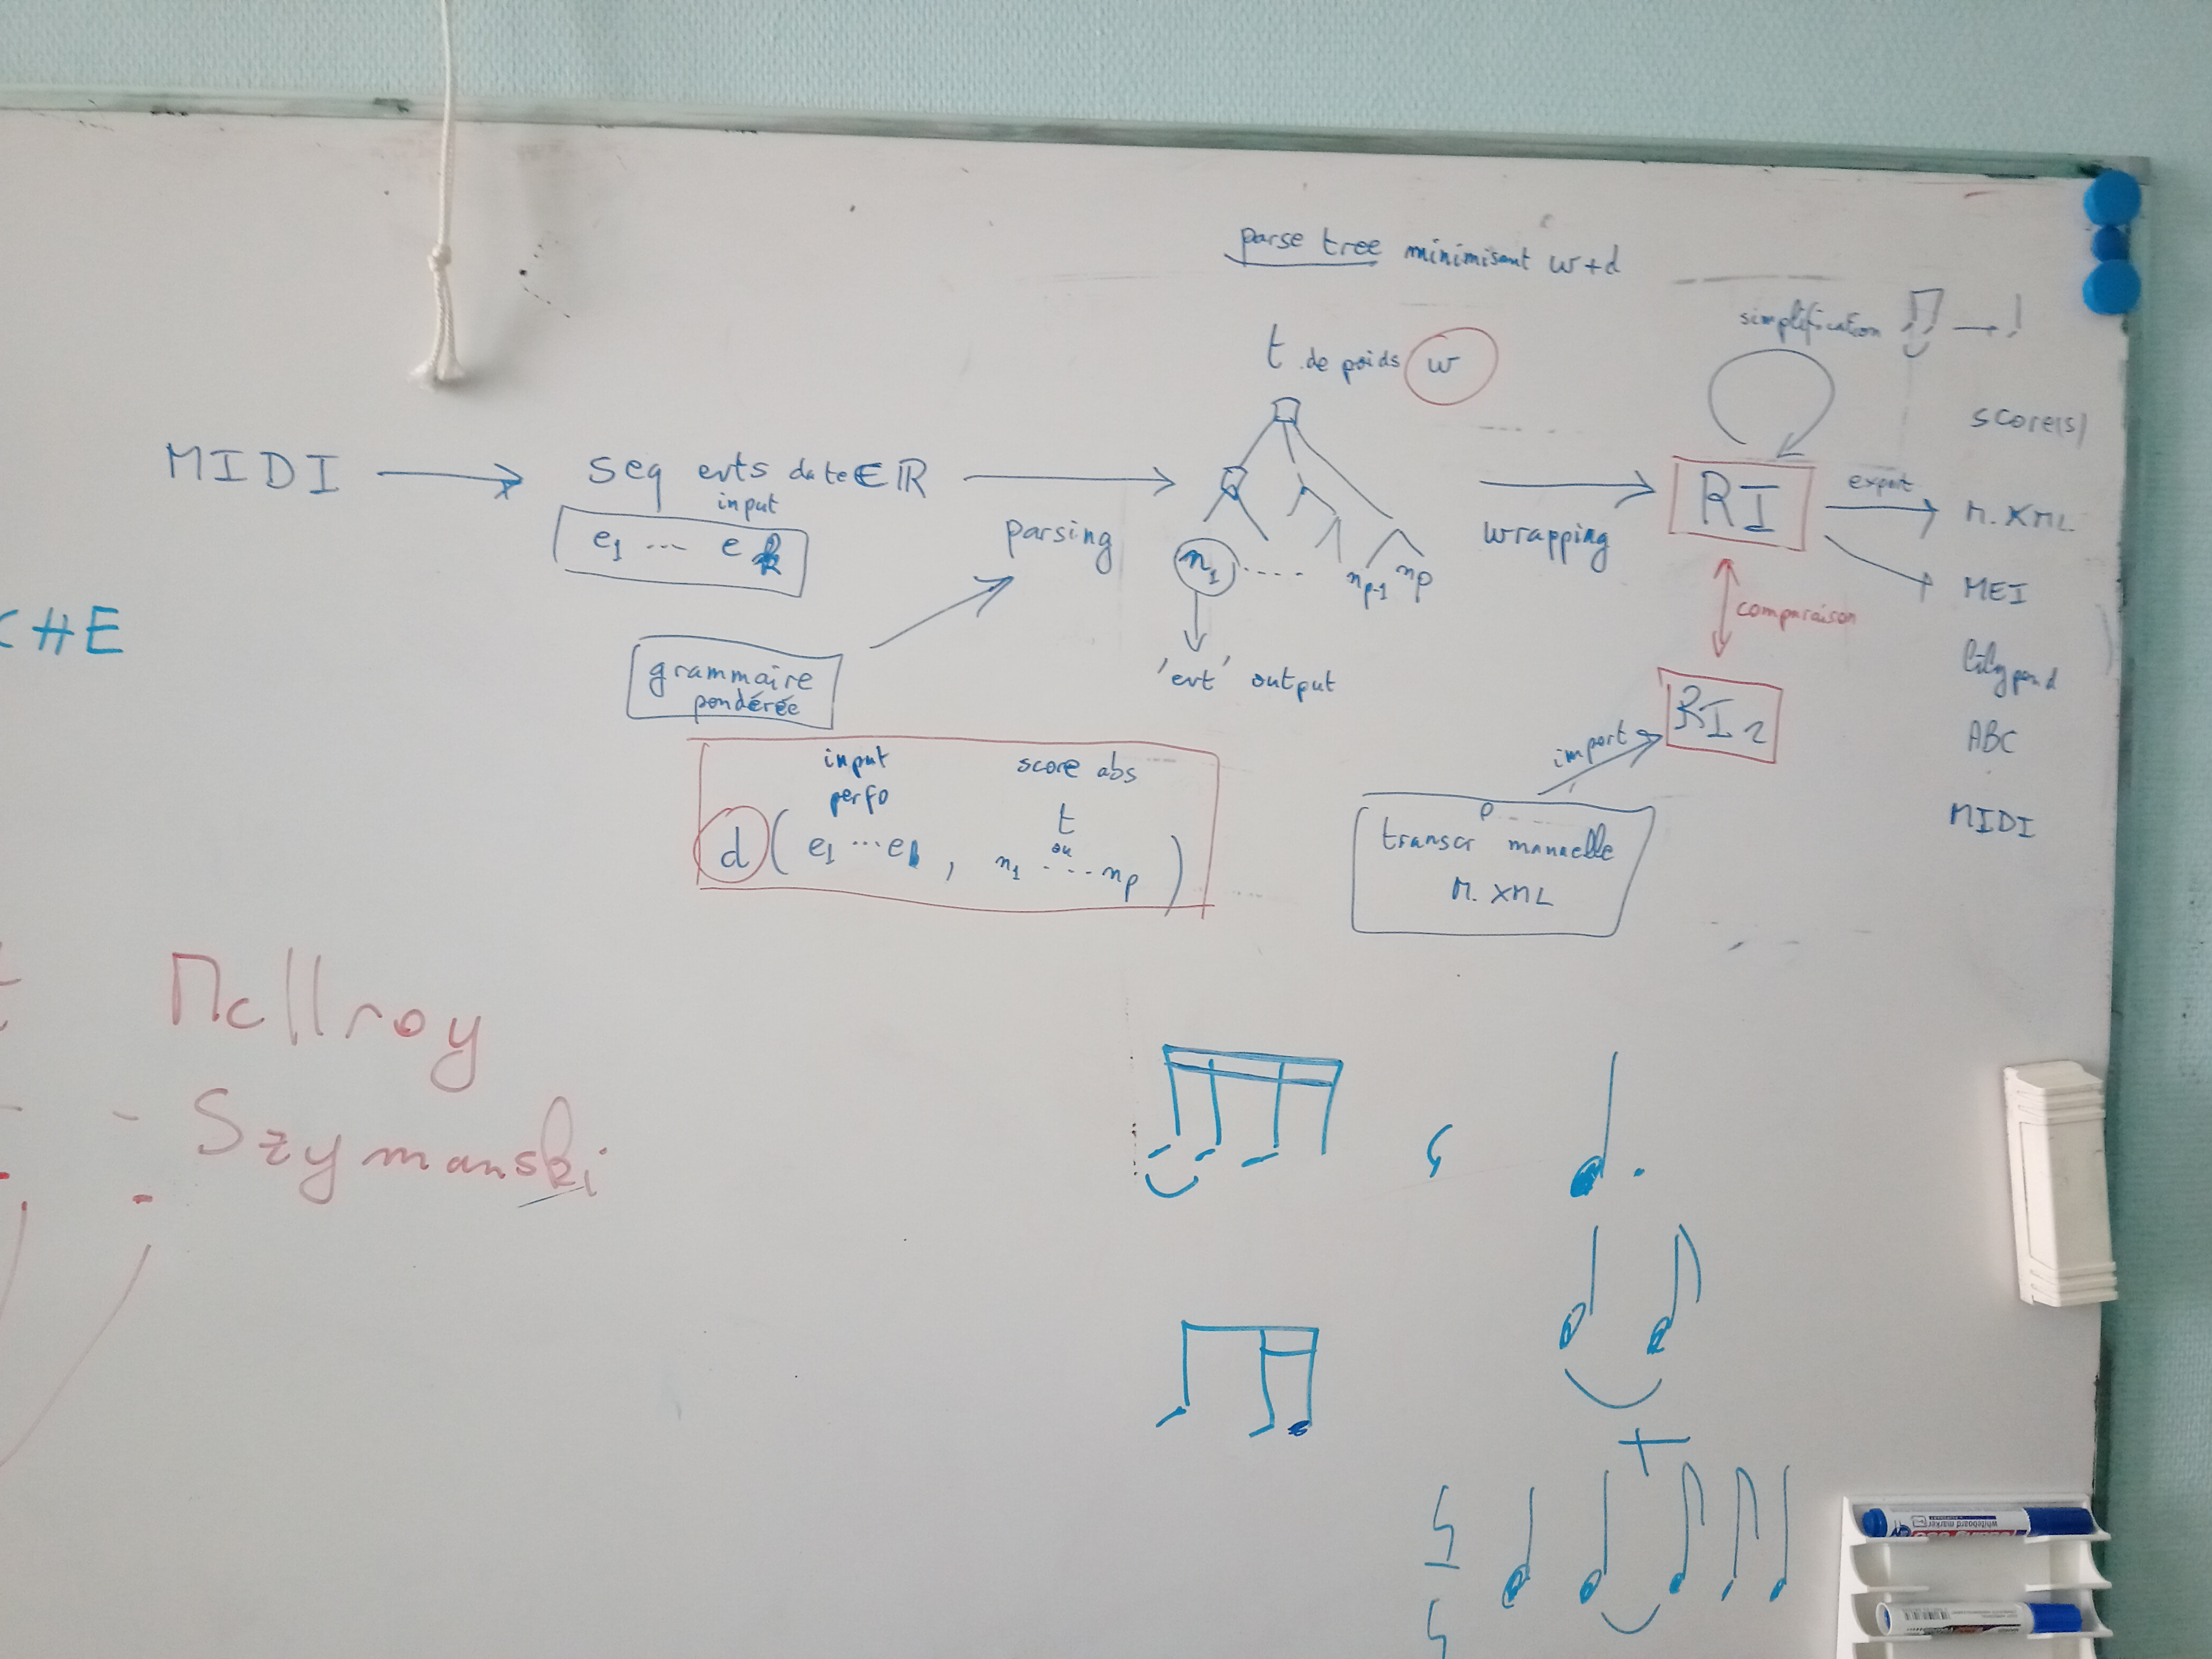
\includegraphics[height=80mm, width=80mm]{images/sujet_stage.jpg} \\\\
	En entrée : midi (séquence d’événements datés (piano roll) accompagné d’une grammaire pondérée)\\
	$\Rightarrow$ parsing\\
	$\Rightarrow$ global parsing tree\\
	$\Rightarrow$ RI (Représentation Intermédiaire) arbres locaux par intruments\\
	$\Rightarrow$ Sortie (xml, mei, lilypond,… )\\
	Minimiser la distance entre le midi et la représentation en arbre.\\\\
	Le but du stage est d’améliorer qparse, un outil de transcription et d’écriture automatique de la batterie (entre autre)\\\\
	\textbf{Le sujet de ce mémoire est de proposer une tâche de reconnaissance du regroupement des notes par les ligatures dans l’écriture de la batterie.}\\\\
	Pour cela, nous utiliserons la logique des systèmes (selon la définition agostinienne).\\$\Rightarrow$ Motif répétitif de plusieurs instruments coordonnées accompagnés d’un texte varié joué par un autre instrument de la batterie.\\\\Nous partirons de propositions génériques de systèmes (environs trois systèmes dans différents style de batterie) que nous tenterons de détecter dans le jeu de données groove.\\\\
	Nous travaillerons aussi sur la détection de répétitions sur plusieurs mesures afin de pouvoir corriger des erreurs sur une des mesures qui aurait dû être identique au autres mais qui présente des différences.
	
	
	


%%%%%%%%%%%%%%%%%%%%%%%%%%%%%%%%%%%%%%%%%%%%%%%%%%%%%%
%% INTRODUCTION
%%%%%%%%%%%%%%%%%%%%%%%%%%%%%%%%%%%%%%%%%%%%%%%%%%%%%%


\chapter*{Introduction}
\adjustmtc
\addstarredchapter{Introduction} 

%% TODO: remplacer ce contenu par le vôtre...
\section*{Pr\'esentation g\'en\'erale}

étonnant non ?

Ce document donne un modèle possible pour rédiger un mémoire sous
\LaTeX{}. Il donne quelques informations sur les commandes les plus
utiles. Ce modèle est inspiré de celui utilisé pour les rapports de
M2R à l'université Paris Sud, complété par des fonctionnalités
pratiques (mini table des matières au début de chaque chapitre, liens
cliquables et colorés pour les références, etc.). Il est évident que
vous n'êtes pas obligés de rédiger votre mémoire sous \LaTeX{}. Si
vous préférez le faire sous un autre éditeur de texte, c'est tout à
fait possible.

Ouvrir le fichier \og{}modele.tex\fg{} avec un éditeur de texte, et
effectuer les modifications nécessaires (cf. lignes qui commencent par
TODO). Les commandes pour compiler les fichiers sont dans
\og{}lanceur.sh\fg{} (voir section~\ref{sec:compilation}).


\section*{Plan de lecture}
Un mémoire de recherche ou un article scientifique se composent
généralement\footnote{Il est accepté que vous, ou votre directeur de
  mémoire, estimiez qu'une autre organisation s'impose pour votre
  problématique de recherche.} des chapitres suivants~:
%
\begin{itemize}
\item Introduction~: présentation générale du contexte et de la
  problématique traitée, plan suivi dans le mémoire~;
\item \'Etat de l'art (chapitre~\ref{chap:articles})~: les articles
  qui traitent du même sujet que vous, présentés en un tout cohérent
  \emph{(extraire de chaque article lu les points essentiels et
    présenter dans ce chapitre le résultat de ces lectures en
    regroupant les articles par point essentiel)}~;
\item Corpus (chapitre~\ref{chap:corpus})~: le corpus utilisé
  \emph{(caractéristiques, pré-traitements appliqués)}~;
\item Méthodes (chapitre~\ref{chap:methodes})~: les méthodes
  appliquées, avec le détail des expériences réalisées (différentes
  configurations)~;
\item Résultats (chapitre~\ref{chap:resultats})~: les résultats
  obtenus sur chacune des expériences~;
\item Discussion (chapitre~\ref{chap:discussion})~: la discussion des
  résultats obtenus (quelle expérience a produit les meilleurs
  résultats, de manière globale, dans le détail des catégories) avec,
  si possible, une analyse des erreurs pour comprendre les
  possibilités d'amélioration~;
\item Conclusion~: la conclusion globale du mémoire.
\end{itemize}

En règle générale, l'introduction et la conclusion sont les deux
sections de contenu à ne pas être numérotées. Idéalement, chaque
chapitre commence par une introduction rapide et se termine par une
conclusion rapide pour aider le lecteur à mémoriser et comprendre ce
qui a été fait.




%%%%%%%%%%%%%%%%%%%%%%%%%%%%%%%%%%%%%%%%%%%%%%%%%%%%%%%%%%%%%%%%
%% Première partie

\part{Contexte général}



%%%%%%%%%%%%%%%%%%%%%%%%%%%%%%%%%%%%%%%%%%%%%%%%%%%%%%
%% ÉTAT DE L'ART
%%%%%%%%%%%%%%%%%%%%%%%%%%%%%%%%%%%%%%%%%%%%%%%%%%%%%%

%% Nota Bene : il est possible de stocker chaque chapitre dans un
%% fichier *.tex distinct (par exemple pour ce chapitre, de la
%% commande \chapter{} jusqu'à la conclusion de ce chapitre) nommé,
%% par exemple "chapitre-etat-art.tex" qui sera appelé au moyen de la
%% commande suivante (la compilation du fichier *.tex principal
%% compile automatiquement les fichiers inclus) :
%%
%% \include{chapitre-etat-art}

\chapter{\'Etat de l'art}
\label{chap:articles}

%% Ajustement de la mini table des matières du fait de l'introduction
%% non numérotées qui introduit un décalage
\adjustmtc
\minitoc



%%%
% Introduction

\section{Introduction}
Dans ce chapitre, nous présentons...


%%%
% Contenu

\section{Contenu}
Une section dans ce chapitre avec un appel cliquable de référence
bibliographique~\cite{grouin-2014jbi}.


%%%
% Conclusion

\section{Conclusion}
Conclusion de ce chapitre.




%%%%%%%%%%%%%%%%%%%%%%%%%%%%%%%%%%%%%%%%%%%%%%%%%%%%%%
%% MÉTHODES
%%%%%%%%%%%%%%%%%%%%%%%%%%%%%%%%%%%%%%%%%%%%%%%%%%%%%%


\chapter{Méthodes}
\label{chap:methodes}

\minitoc


%%%
% Introduction

\section{Introduction}
Dans ce chapitre...


%%%
% Contenu

\section{Contenu}
Une section dans ce chapitre...
\subsubsection*{Propositions de règles de ré-écriture}
Basé sur \cite{jacquemard:hal-01134096} et sur \cite{jacquemard:hal-01403982}
Pour la plupart des instruments mélodiques, la liaison et le point sont les deux seules possibilités en cas d’équivalence rythmique. Mais la batterie offre un 3ème choix pour combler la distance rythmique entre deux notes : les silences.\\Les cymbales-crash et les ouvertures de charley constituent le seul cas qui exclut cette option. Le charley car ses ouvertures/fermetures sont presque toujours quantifiées. Les fermetures du charley sont notées soit par un silence (correspondant à une fermeture de la pédale), soit par un écrasement de l’ouverture par un autre coup de charley fermé, au pied ou à la main.
\begin{itemize}
\item 
Tie to dot devient Tie to note\&rest\\
par exemple : une noire liée à une autre noire devient une noire + un soupir.\\
On remplace donc la dernière note d’une liaison par sa valeur en silence.
Ceci ne concerne pas les ouvertures de charley, qui sont, avec les cymbales-crash, les seuls indications sonores dont nous considèrerons la durée.
\item 
Dans tous les cas, sauf ouverture de hh-pd, Une note sur un temps suivie d’une note en l’air sur le second temps seront écrites : noire sur le temps 1 puis silence + note pertinente sur le temps 2.
\item
Pour un charley ouvert qui déborde sur le temps d’après, le choix le plus pertinent est-il la note pointée ou la liaison ? Je pense que c’est la liaison car il marchera même dans les cas où le point ne marche pas (ex : mauvaise durée)
\item
une blanche sera écrite noir + soupir.\\
Voir exemples dans :
Stage\_M2\_Inria/2\_Transcriptions\_LilyPond/exemples\_rewriting
\end{itemize}

Les deux instruments qui seront difficiles à placer seront la caisse claire et le charley au pied car ils ne seront pas toujours affiliés aux mêmes instruments.

%%%
% Conclusion

\section{Conclusion}
Conclusion de ce chapitre.




%%%%%%%%%%%%%%%%%%%%%%%%%%%%%%%%%%%%%%%%%%%%%%%%%%%%%%%%%%%%%%%%
%% Deuxième partie

\part{Expérimentations}



%%%%%%%%%%%%%%%%%%%%%%%%%%%%%%%%%%%%%%%%%%%%%%%%%%%%%%
%% CORPUS
%%%%%%%%%%%%%%%%%%%%%%%%%%%%%%%%%%%%%%%%%%%%%%%%%%%%%%


\chapter{Corpus}
\label{chap:corpus}

\minitoc


%%%
% Introduction

\section{Introduction}
Dans ce chapitre...


%%%
% Contenu

\section{Contenu}
Une section dans ce chapitre...


%%%
% Conclusion

\section{Conclusion}
Conclusion de ce chapitre.




%%%%%%%%%%%%%%%%%%%%%%%%%%%%%%%%%%%%%%%%%%%%%%%%%%%%%%
%% RÉSULTATS
%%%%%%%%%%%%%%%%%%%%%%%%%%%%%%%%%%%%%%%%%%%%%%%%%%%%%%


\chapter{Résultats}
\label{chap:resultats}

\minitoc


%%%
% Introduction

\section{Introduction}
Dans ce chapitre...


%%%
% Contenu

\section{Contenu}
Une section dans ce chapitre...


%%%
% Conclusion

\section{Conclusion}
Conclusion de ce chapitre.




%%%%%%%%%%%%%%%%%%%%%%%%%%%%%%%%%%%%%%%%%%%%%%%%%%%%%%
%% DISCUSSION
%%%%%%%%%%%%%%%%%%%%%%%%%%%%%%%%%%%%%%%%%%%%%%%%%%%%%%


\chapter{Discussion}
\label{chap:discussion}

\minitoc


%%%
% Introduction

\section{Introduction}
Dans ce chapitre...


%%%
% Contenu

\section{Contenu}
Une section dans ce chapitre...


%%%
% Conclusion

\section{Conclusion}
Conclusion de ce chapitre.




%%%%%%%%%%%%%%%%%%%%%%%%%%%%%%%%%%%%%%%%%%%%%%%%%%%%%%
%% CONCLUSION
%%%%%%%%%%%%%%%%%%%%%%%%%%%%%%%%%%%%%%%%%%%%%%%%%%%%%%


\cleardoublepage\pdfbookmark[-1]{Conclusion générale}{conclusion} %% CG: lien dans le PDF hors d'une partie
\chapter*{Conclusion générale}
\adjustmtc
\addstarredchapter{Conclusion générale} 

Dans ce mémoire, nous avons traité de la problématique...







% ================================== BIBLIOGRAPHIE =============================

\cleardoublepage\pdfbookmark[-1]{Bibliographie}{bibliography}
%\selectlanguage{english} 
\bibliographystyle{apalike} % style alphabétique en français
\bibliography{biblio_utf8} % pour afficher la biblio
\selectlanguage{french} 




\appendix
\cleardoublepage\pdfbookmark[-1]{Annexes}{appendix}
%% TODO: mettre en commentaires les annexes, ou remplacer l'appel de
%% fichier *.tex par votre fichier d'annexe.
\chapter{Documentation}

\section{Compilation}
\label{sec:compilation}
La compilation d'un fichier \LaTeX{} nommé \og{}modele.tex\fg{} se fait au moyen des étapes suivantes (en lignes de commande)~:
%
\begin{itemize}
\item \verb+pdflatex modele+ (première compilation pour l'appel des différentes fonctionnalités contenues dans le mémoire)~;
\item \verb+bibtex modele+ (préparation de la bibliographie)~;
\item \verb+makeindex modele+ (préparation de l'index)~;
\item \verb+pdflatex modele+ (à faire 2 fois, produit le PDF complet).
\end{itemize}



%%%
% Images

\section{Les images}
\label{sec:images}

Le \index{Schéma} schéma~\ref{fig:schema} présente le schéma
d'annotation en entités nommées du domaine biomédical que nous avons
utilisé pour annoter nos corpus de données.
%
\begin{figure}[h]
  \centering
  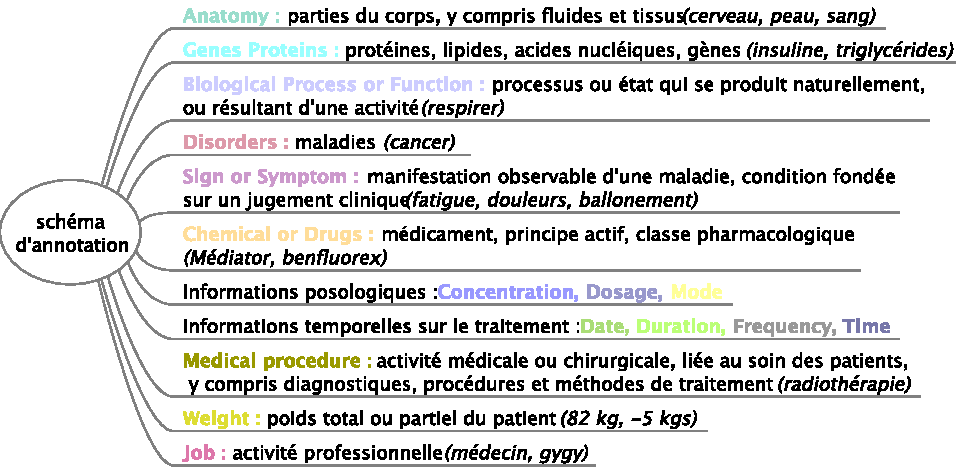
\includegraphics[width=.8\linewidth]{annotation2.pdf}
  \caption{Schéma d'annotation défini pour les entités nommées
    biomédicales}
  \label{fig:schema}
\end{figure}

L'intégration d'une image (format PDF, PNG) se fait au moyen de la
commande \verb+\includegraphics{fichier.pdf}+ avec d'éventuelles
options entre crochets pour spécifier la taille de l'image (height,
width) par rapport à la page.


%%%
% Tableaux

\newpage
\section{Les tableaux}
\label{sec:tableaux}

Pour réaliser un \index{Tableau} tableau en \LaTeX{}, la syntaxe
ressemble à (voir tableau~\ref{tab:exemple})~:
%
\begin{table}[h]
  \centering
  \begin{tabular}{|l|c|c|r|} \hline
    Expérience & Rappel & Précision & F-mesure \\ \hline
    Baseline & 0,372 & 0,500 & 0,427 \\
    Lexique & 0,907 & 0,903 & 0,905 \\
    Apprentissage & 0,880 & 0,942 & 0,910 \\ \hline
  \end{tabular}
  \caption{Résultats généraux pour chaque expérience}
  \label{tab:exemple}
\end{table}

Dans la commande \verb+\begin{tabular}{|l|c|c|r|}+ on définit le
  nombre de colonnes (ici 4), la manière dont le texte est mis en
  forme dans chaque colonne (l=left, c=center, r=right), et le
  séparateur de colonne (ici une ligne verticale). La commande
  \verb+\hline+ permet de tracer une ligne horizontale. La commande
  \verb+\caption{Titre ou légende}+ permet de définir la légende d'un
  tableau. Et la commande \verb+\label{nom}+ permet de nommer le
  tableau pour le désigner dans le corps du texte avec la commande
  \verb+\ref{nom}+ (e.g., tableau~\ref{tab:exemple}).

Les commandes \verb+\multirow{n}{*}{Texte}+ et
\verb+\multicolumn{n}{c}{Texte}+ permettent de fusionner plusieurs
lignes et plusieurs colonnes, avec $n$ le nombre de lignes ou colonnes
fusionnées. La commande \verb+\cline{2-4}+ permet de dessiner une
ligne horizontale de la colonne 2 à la colonne 4 (voir tableau~\ref{tab:autre}).
%
\begin{table}[h]
  \centering
  \begin{tabular}{|l|ccc|} \hline
    \multirow{2}{*}{Expérience} & \multicolumn{3}{c|}{Mesures} \\ \cline{2-4}
    & Rappel & Précision & F-mesure \\ \hline
    Baseline & 0,372 & 0,500 & 0,427 \\
    Lexique & 0,907 & 0,903 & 0,905 \\
    Apprentissage & 0,880 & 0,942 & \textbf{0,910} \\ \hline
  \end{tabular}
  \caption{Fusion de lignes et de colonnes dans un tableau}
  \label{tab:autre}
\end{table}


%%%
% Mise en forme

\section{Mise en forme}
\index{Mise en forme}
Il est possible de mettre du texte en \emph{emphase}
\verb+\emph{texte}+, en \textsl{version penchée}
\verb+\textsl{texte}+, en \textbf{gras} \verb+\textbf{texte}+, en
version \textsf{Sans Serif} (similaire à Arial et Helvetica)
\verb+\textsf{texte}+ ou encore en \textsc{Petites Capitales}
\verb+\textsc{Texte}+. Il n'est pas recommandé d'utiliser le
\underline{souligné} au vu de l'effet produit. Pour ajouter une note
de bas de page\footnote{Les notes de bas de page sont numérotées
  automatiquement en fonction de leur utilisation tout au long du
  texte. Avec ce modèle, la numérotation est remise à 1 à chaque début
  de chapitre.}, on utilise la commande
\verb+\footnote{Contenu}+. L'espace insécable (c.-à-d. qui ne peut pas
être coupée si elle est en fin de ligne), est représentée par le
tilde. On l'utilise généralement avant un appel de référence, ou avant
la référence d'un tableau ou d'une figure \verb+Tableau~\ref{clé}+.

Il est possible de ne pas numéroter les titres de section,
sous-section, etc., en utilisant la commande
\verb+\section{Titre}+. Dans ce cas, il est nécessaire d'ajuster les
mini tables des matières qui figurent au début de chaque chapitre au
moyen de la commande \verb+\adjustmtc+ en intégrant cette commande
autant de fois que nécessaire avant la commande \verb+\minitoc+

Pour forcer un saut de page, on utilise la commande \verb+\newpage+ et
pour un saut de ligne \verb+\\+


%%%
% Formules mathématiques

\section{Formules mathématiques}
\index{Rappel} Le rappel (formule~\ref{form:rappel}) mesure le nombre
d'éléments correctement étiquetés par le système (vrais positifs)
rapporté au nombre d'éléments étiquetés dans la référence (vrais
positifs et faux négatifs).
%
\begin{equation}
  \centering
  \text{Rappel} = {{\text{vrais positifs}}\over{\text{vrais positifs + faux négatifs}}}
  \label{form:rappel}
\end{equation}

\index{Precision@Précision} La précision
(formule~\ref{form:precision}) mesure le nombre d'éléments
correctement étiquetés par le système (vrais positifs) rapporté au
nombre total d'éléments étiquetés par le système (vrais et faux
positifs).
%
\begin{equation}
  \centering
  \text{Précision} = {{\text{vrais positifs}}\over{\text{vrais positifs + faux positifs}}}
  \label{form:precision}
\end{equation}

\index{F-mesure} La F-mesure (formule~\ref{form:fmesure}) est la
moyenne harmonique pondérée du rappel et de la précision. La valeur
accordée à $\beta$ permet de pondérer le rappel ou la précision, ou
d'équilibrer les deux mesures (avec $\beta=1$).
%
\begin{equation}
  \centering
  \text{F-mesure} = {{(1+\beta^2) \times \text{ précision } \times \text{ rappel }}\over{\beta^2 \times \text{ précision } + \text{ rappel } }}
  \label{form:fmesure}
\end{equation}

Les plus motivés d'entre vous pourront également réaliser des figures
(arbre syntaxique, histogramme, diagramme circulaire, etc.)
directement sous \LaTeX{} en utilisant le package Tikz\footnote{Voir
  \url{http://bertrandmasson.free.fr/index.php?categorie6/latex-pgf-tikz}
  pour de nombreux exemples utiles.} une fois qu'ils auront terminé la
rédaction de leur mémoire pour ne pas perdre de temps dès le départ...


%%%
% Bibliographie

\section{Gestion de la bibliographie}
La \index{Bibliographie} bibliographie figure dans un fichier nommé
\og{}biblio.bib\fg{}. Ce fichier peut être édité dans un éditeur de
texte classique \emph{(emacs, vi, notepad)}, ou par le biais d'un
outil de gestion de bibliographie tel que \textsf{JabRef}, un
programme Java qui permet de gérer efficacement les fichiers *.bib et
de remplir les différents champs nécessaires à chaque entrée.

\subsection{Appels de référence}
On appelle les références au moyen de la
commande \verb+\cite{clé}+ avec une clé de citation qui est définie
dans la bibliographie. On intègre généralement une référence
bibliographique après avoir introduit le concept. Par exemple~: nos
expériences en approche statistique reposent sur le formalisme des
CRF~\cite{lafferty-2001icml} implémenté dans l'outil
WAPITI~\cite{lavergne-2010acl}. Nous avons suivi le protocole défini
par~\cite[p.~3]{grouin-2014jbi} pour constituer les annotations de corpus.

Il est possible de citer plusieurs articles en même temps en séparant
chaque clé par une virgule. Par exemple~: notre travail repose sur la
détection d'entités nommées~\cite{ehrmann2008phd, sekine-2009} du
domaine biomédical, en particulier la détection des mentions de
bactéries et de biotopes~\cite{bossy-2012bb}.


\subsection{Format}
\LaTeX{} gère automatiquement le format de présentation des
références, selon que l'article cité a été rédigé par un
auteur~\cite{ehrmann2008phd} (auquel cas sont mentionnés le nom et
l'année), deux auteurs~\cite{bretonnel-2008plos} (les noms des deux
auteurs et l'année), ou plus de deux auteurs~\cite{brown-1992cl} (le
nom du premier auteur, la mention \emph{et al.}\footnote{Locution
  latine signifiant \og{}et d'autres\fg{}.}, et l'année).


\chapter{Principes à suivre}

\section{Le sujet de votre mémoire}
Vous avez acquis, au cours de l'année 2015-2016, des compétences d'ingénieur-linguiste ; vous savez donc analyser un problème, proposer une méthodologie permettant d'arriver à une solution et montrer les limites de cette dernière. C'est cette démarche qui constituera le fil directeur de votre mémoire.

Ce travail devra être original et personnel. Le cadre de votre travail est naturellement la linguistique et, étant donné le diplôme que vous préparez, la linguistique appliquée, plutôt que théorique. Ceci ne veut néanmoins pas dire que vous ne devrez pas situer votre démarche à l'intérieur d'un cadre théorique, au contraire. On souhaite cependant que ce cadre serve d'appui à la création ou à la transformation d'outils, à la mise au point de méthodologies vous permettant de proposer un résultat.

Cela revient à dire que votre mémoire constitue une tentative de problématiser une approche méthodologique, de proposer une piste nouvelle, de comparer des méthodes, des outils, etc. Il contiendra en tout cas un état de l'art et s'appuiera sur une bibliographie précise et récente. L'état de l'art ne doit pas être déconnecté de la question traitée : on ne vous demande pas de \og{}faire un état de l'art pour faire un état de l'art\fg{} mais, au contraire, de montrer comment se situe votre travail par rapport à cet état de l'art.
Si votre sujet s'y prête, et afin d'en faciliter la réalisation, vous pouvez segmenter votre état de l'art en plusieurs parties ciblées à placer en tête des chapitres correspondant plutôt que d'écrire un chapitre consacré qui risque d'être généraliste et donc insuffisamment précis.

Vous devrez avoir choisi un sujet de mémoire à la mi-mai ou, à tout le moins, avoir réfléchi à des pistes sérieuses. Vous devrez vous assurer auprès d'un intervenant du TIM/ER-TIM que vous ne faites pas fausse route et que votre mémoire ne sera pas hors-sujet. Il s'agit d'éviter que vous ne traitiez un sujet dont les exigences techniques pourraient s'avérer supérieures à ce que vous croyez connaître. Le(s) stage(s) de fin d'études que vous devez entreprendre peu(t/vent) vous aider à affiner votre choix de sujet, mais vous devez garder à l'esprit que votre mémoire ne doit pas se confondre avec une description de votre stage. Notez bien que les rapports de stage ne sont pas pris en compte dans l'évaluation de votre Master.

Pour vous aider, vous pouvez consulter les meilleurs mémoires des années précédentes (et dont les résumés sont en ligne sur le site \url{www.er-tim.fr}). \'Evidemment, vous consulterez également les articles scientifiques liés à votre problématique : outre les connaissances que vous pourrez ainsi acquérir, cela vous permettra aussi de vous familiariser avec ce genre bien spécifique. Si vous ne trouviez pas de sujet vous permettant de mettre en pratique les connaissances acquises au cours de cette année, en fonction de vos goûts et attentes personnels ou professionnels, nous vous en proposerions un (consultez-nous, donc).

\section{L'encadrement du mémoire}
Vous avez toute latitude pour choisir, selon affinités, la/les personne(s) qui va/vont diriger vos recherches. Mais un/des intervenant(s) du TIM/ER-TIM figurera/ont nécessairement dans votre jury lors de la soutenance. Il faut donc nécessairement avoir pris contact avec ces personnes et s'assurer de leur collaboration. Si vous envisagez de faire une thèse ensuite, il est recommandé de solliciter un enseignant assimilé professeur ou habilité à diriger des recherches ou de mettre en place un co-encadrement en ce sens.

En règle générale, le TIM/ER-TIM souhaite, autant que faire se peut, que les personnes qui vous ont encadré lors de votre stage et qui ont pu vous conseiller pour la rédaction de votre mémoire, soient présentes lors de la soutenance. Elles apportent un complément d'information interne sur le stage et les conditions de réalisation du mémoire, éclairage qui peut être tout à fait pertinent.

Si vous rencontrez des problèmes et souhaitez poser des questions, il est impératif, dans un premier temps, de les formuler par courrier électronique plutôt que de venir immédiatement au TIM/ER-TIM, riche en compétences mais pauvre en personnel. Par ailleurs, vous ne devez pas envoyer par courrier électronique des centaines de pages à fin de re-lecture : lorsqu'une pré-version de votre travail vous semblera digne de relecture, déposez-la au TIM/ER-TIM, ou postez-la.

\section{L'évaluation du mémoire}
L'évaluation du mémoire est fonction de la qualité de votre travail écrit et de votre capacité à répondre aux questions, remarques, critiques qui peuvent vous être adressées pendant la soutenance. La qualité du travail écrit dépend de plusieurs critères, dont voici une liste non-exhaustive :
\begin{itemize}
\item votre mémoire forme-t-il un ensemble cohérent qui doit son unité à la volonté de répondre à une problématique bien définie ?
\item votre mémoire est-il réutilisable par une personne souhaitant faire un bilan de la problématique soulevée, tant du point de vue fond que forme (clarté de la bibliographie, description en annexe des outils utilisés avec liens aux sources, disponibilités des sources sur le CD-ROM d'accompagnement de votre mémoire, index permettant une consultation rapide, table des matières, pagination, etc.) ?
\item votre mémoire répond-t-il vraiment à l'objectif fixé au départ ? le titre de votre mémoire correspond-il vraiment au contenu ? les mots-clés qui seront mis en ligne sont-ils pertinents ?
\item votre mémoire met-il en valeur un angle de vue original sur un savoir-faire classique ?
\item votre mémoire parvient-il à mettre la théorie à l'épreuve ? \^Etes-vous capable de fournir des résultats, des exemples, un bilan d'expérience, des critères d'évaluation, une évaluation ?
\item la bibliographie doit être totalement normalisée, de façon à permettre une consultation aisée, les annexes contiendront un descriptif pratique et les références des outils utilisés, un échantillon des corpus utilisés et des programmes que vous avez écrits et, de manière générale, tout ce qui peut illustrer le travail réalisé. Attention, pour des raisons de place, vous ne devez évidemment pas présenter tous vos corpus et tous vos programmes en annexe, mais un simple échantillon. En revanche, corpus\footnote{Vérifiez toutefois que vous avez le droit de reproduire tout ou partie du corpus sur lequel vous aurez travaillé, en particulier pour les corpus de documents cliniques.} et programmes figureront impérativement et exhaustivement sur le CD fourni.
\end{itemize}

La qualité de votre prestation orale est importante. Vous devrez vous assurer, en particulier, que :
\begin{itemize}
\item vous savez vous affranchir du plan de votre mémoire mais vous devez néanmoins faire un bref résumé de la problématique car tous les membres du jury n'auront pas lu votre mémoire
\item vous donnez des exemples concrets des questions qui se sont posées et des solutions apportées, de façon à montrer que vous ne traitez pas le sujet de façon purement théorique
\item vous savez situer la problématique de votre mémoire par rapport aux travaux les plus connus et les plus récents sur la question
\item vous savez faire le lien entre les connaissances acquises au cours de l'année et la mise en pratique de ces connaissances lors de la réalisation du mémoire
\item vous savez répondre aux questions ou critiques qui vous sont soumises
\end{itemize}

\section{La démarche à suivre pour soutenir}
Trois semaines avant la date de soutenance, vous devez envoyer une version présentable de votre mémoire à votre encadrant et à l'équipe de formation, pour déterminer si le mémoire est soutenable. Vous devez remettre une version papier définitive de vos mémoires au moins 15 jours avant la soutenance.
\begin{itemize}
\item La soutenance pour la première session est fixée entre le 20 et le 24 juin 2016 (à préciser) pour ceux d'entre vous qui candidateraient à un contrat doctoral INaLCO (voir la procédure sur le site \url{www.inalco.fr}, le comité de sélection ayant lieu le 1 juillet 2016).
\item Pour la deuxième session (inscription en doctorat à l'INaLCO selon la procédure normale), la soutenance est fixée le 30 septembre 2016.
\item Pour la dernière session, la date de soutenance est fixée le 18 novembre 2016.
\end{itemize}

Vous devez déposer votre travail au moins deux semaines avant d'espérer soutenir. Il faut en effet qu'il soit lu, puis, si nécessaire, amendé et corrigé -- voire rejeté et réécrit -- de façon que la soutenance ne verse pas dans la critique systématique.

Au plus tard la veille de votre soutenance, vous aurez envoyé à \url{crim@inalco.fr} et à \url{sophie.urbaniak@inalco.fr} un résumé de votre mémoire de 10 lignes maximum ainsi que 5 mots-clés permettant de situer votre travail. Attention, ces informations sont destinées à être consultées et doivent donc être le reflet fidèle de votre travail final.

Une fois votre travail accepté, nous vous proposerons un ordre de passage pour la soutenance. Vous devrez fournir 3 exemplaires/support-papier et 3 exemplaires/support-électronique de votre mémoire (ces exemplaires sont destinés aux membres du jury et aux futurs étudiants). Sur le 4ème de couverture vous agraferez une enveloppe format 21-27 qui contiendra le CD correspondant à votre travail. Ce CD contiendra, outre la version électronique de votre mémoire, toutes les annexes ne pouvant figurer dans le mémoire pour des raisons de place : corpus, code source des outils utilisés, polices de caractères utilisées, code des programmes que vous avez élaborés.







% =============================== INDEX DES NOTATIONS ==========================

\cleardoublepage % pour forcer l'index à apparaître sur une page impaire
\pdfbookmark[-1]{Index}{index}
\printindex % pour afficher l'index



%% \newpage
%% \thispagestyle{empty}
%% \mbox{}


\end{document}
